\documentclass[12pt]{article}
\usepackage{graphicx}
\usepackage{float}
\usepackage{ragged2e}
\usepackage{setspace}
\usepackage[usestackEOL]{stackengine}
\usepackage{listings}
\usepackage{color}
\usepackage{subcaption}
\usepackage{polyglossia}
\usepackage{fontspec}
\setdefaultlanguage{english}
\setotherlanguage{sanskrit}
\newfontfamily\devanagarifont[Script=Devanagari]{Lohit-Devanagari.ttf}

\definecolor{dkgreen}{rgb}{0,0.6,0}
\definecolor{gray}{rgb}{0.5,0.5,0.5}
\definecolor{mauve}{rgb}{0.58,0,0.82}

\lstset{frame=tb,
	language=Python,
	aboveskip=3mm,
	belowskip=3mm,
	showstringspaces=false,
	columns=flexible,
	basicstyle={\small\ttfamily},
	numbers=none,
	numberstyle=\tiny\color{gray},
	keywordstyle=\color{blue},
	commentstyle=\color{dkgreen},
	stringstyle=\color{mauve},
	breaklines=true,
	breakatwhitespace=true,
	tabsize=3
}

\onehalfspace
\begin{document}
	\title{\textbf{Search Engine for Indian Languages}}
	\date{}
	\maketitle
	\centering{Project Report\\}
	\centering{Submitted in partial fulfilment of\\}
	\centering{\textbf{Bachelor of Technology(Hons.)}\\}
	\centering{in\\}
	\centering{\textbf{Computer Science and Engineering}\\}
	\centering{by\\}
	\centering{\textbf{Shubham Kumar (2017UGCS001R)}\\}
	\centering{Under the guidance of\\}
	\centering{\textbf{Dr. Jayadeep Pati}}
	\begin{figure}[H]
		\centering
		
\includegraphics[width=4cm, height=3cm]{logo.jpeg}
	\end{figure}
	\centering{\textbf{Department of Computer Science and Engineering\\}}
	\centering{\textbf{Indian Institute of Information Technology, Ranchi}\\}
	\centering{\textbf{Jharkhand - 834010}\\}
	\centering{\textbf{India}}
	\pagenumbering{gobble}
	
	\pagebreak
	
	\centering{\Large{\textbf{CANDIDATE'S DECLARATION}}\\}
	\smallskip
	\smallskip
	\justifying{
		I hereby declare that the work which is being presented in the project titled "SEARCH ENGINE FOR INDIAN LANGUAGES" towards the partial fulfillment of the requirements for the award of the degree of Bachelor of Technology (Hons.) in COMPUTER SCIENCE AND ENGINEERING submitted in the Department of Computer Science and Engineering, Indian Institute of Information Technology, Ranchi is an authentic record of my original work carried out during the academic session 2020-2021 under the esteemed guidance of DR. JAYADEEP PATI, Depatment of Computer Science and Engineering, Indian Institute of Information Technology, Ranchi.\\
		To the best of our knowledge, the content of this project work has not been submitted or published anywhere.}
	\smallskip
	\smallskip
	\smallskip
	\smallskip
	\smallskip
	\\
	Date : \hfill Shubham Kumar(2017UGCS001R)\\
	\smallskip
	Place : IIIT Ranchi
	
	
	\pagebreak
	
	
	\centering{\Large{\textbf{CERTIFICATE}\\}}
	\smallskip
	\smallskip
	\justifying{This is to certify that the B.Tech project titled "SEARCH ENGINE FOR INDIAN LANGUAGES" has been done by the student under my supervision during the academic session 2020-21.}
	\smallskip
	\smallskip
	\smallskip
	\smallskip
	\smallskip
	\smallskip
	\smallskip
	\\
	Dr. Jayadeep Pati, \\
	Computer Science and Engineering
	\smallskip
	\smallskip
	\smallskip
	\smallskip
	\smallskip
	\smallskip
	\\
	Date : \\
	Place : IIIT Ranchi
	
	\pagebreak
	
	\centering{\Large{\textbf{ACKNOWLEDGEMENT}}\\}
	\smallskip
	\smallskip
	\smallskip
	\smallskip
	
	\justifying{Firstly, I would like to thank IIIT Ranchi for giving me the opportunity to perform this project. It has been a challenging and learning experience for me to have worked on this project.}\par
	
	\justifying{With great pleasure and respect, I would like to thank my mentor \textbf{Dr. Jayadeep Pati} (Department of Computer Science and Engineering) for his guidance throughout the project. His teachings and assistance has been key to the completion of the project.}\par
	\smallskip
	\smallskip
	\smallskip
	\smallskip
	\smallskip
	{\raggedleft\Longstack[l]{
			Regards,\\
			Shubham Kumar (2017UGCS001R)
		}\par
	}

	\pagebreak
	
	\centering{\Large{\textbf{ABSTRACT}}}\\
	\justifying{Literature in many of the Indian Languages has failed to attract popularity mainly because of the
		reason that literary works in these languages are not easily found on the internet and there is no
		easy way to find them. The present work tries to create a Search Engine for Indian languages like
		Hindi, Bengali and Oriya. Currently, a prototype with the ability to search using only Hindi and
		English is being developed. The documents have been scraped from popular Hindi websites
		containing mythological and inspirational stories using Python. Developing the search engine
		involves various NLP tools like Parts of Speech Taggers and Stemmers
		in the mentioned languages. These tools aid in processing the query before searching for relevant
		documents. The data from the documents to be searched is indexed and stored in a database. When
		a search query is made, the query is processed and matched with the existing indices. The matching
		results are then ranked according to their relevance.}\par
	\pagebreak
	\begin{center}
		\centering{\Large{\textbf{Full Forms}}}
	\end{center}
	\begin{itemize}
		\item DFD: Data Flow Diagram
		\item NLP : Natural Language Processing
		\item TF-IDF : Term Frequency Inverse Document Frequency
		\item API : Application Programming Interface
		\item JSON : JavaScript Object Notation
	\end{itemize}
	\pagebreak
	\tableofcontents
	\pagebreak
	\listoftables
	\pagebreak
	\listoffigures
	\pagebreak
	
	\section{Introduction}
	\pagenumbering{arabic}
	Search Engines have played a crucial role in pushing the human race forward in the Information Age. They have eliminated the hassles of referring to different books everytime a person has the slightest of doubt on a concept. They serve information right at out computer screens, ready to be consumed. Google has been a lifesaver for people from different walks of life like Software Developers looking for code documentation, students trying to learn different concepts or just a normal human being looking for information on sports, news, general knowledge etc.\\
	
	The advent of search engines has given fuel to the bibliophile's ever burning fire; the desire to learn. Indian authors have been prolific in producing texts of spiritual, cultural, historical and scientific importance over millenia. These documents need to be indexed properly and made searchable to make them available to anyone searching for knowlwdge and most importantly, to save them from exitinction. A search engine specializing in Indian languages needs to be developed. This is the aim with which this project has been developed.\\
	
	A search engine has different components, acting in cohesion, to make the mechanism work. Firstly, the documents need to be indexed, in a way similar to how a textbook is indexed. This helps in faster search of the input search-query. It is a preprocessing step that needs to be done after a document is added in the database or generally when the search traffic is not too high. This process is generally computaionally expensive.\\
	
	Secondly, the input query is processed to get a list of the documents matching the search-query. This process generally breaks up the query into smaller tokens and mathces the tokens with the index. The tokens might also undergo some changes during this step.\\
	
	Lastly, a ranking of all the matches is done, so as to serve the documents that are most relevant to the search-query. The documents are ranked according to their importance and displayed to the user.\\
	
	A search engine needs to perform the search as fast as possible and in a way that is least computationally expensive. Scalability and speed are the most important factors to the commercial success of a search engine.
	
	\pagebreak
	
	\section{Related Work}
	Researchers have produced several works targeted at one or more of the three stages of search - indexing, searching and ranking.  \\
	
	In 2018, Rahman, Rupa and Tuhin published a paper - "Implementing a Search Engine for Bangladeshi E-Commerce Product" \cite{ecom}. It tries to develop a fast search engine for the Bangladeshi E-commerce structure. It's first stage is the acquisition of data from various sources on the internet. Then, the data is stored in a Document Data Store. A copy of it undergoes Text Transformation  and finally, index creation. It uses the BM25 score for rank calculation. \\
	
	A paper titled "Design and Implementation of an efficient Search Engine with Bangla using Natural Language Processing" was published by Roy, Sujan and Hasan, Mahmudul \cite{saitama}. Their work had a dynamic Bangla interface which provided the user to enter the query in a user friendly manner. The NLP engine generated a recognizable sentence after query processing. The words were stemmed using a Bangla stemmer and the stemmed word was stored in the index. A similarity score was used to match the search query with the index. Finally, the results were ranked using the PageRank algorithm.\\
	
	Das, Banerjee and Mitra from the Indian Institute of Technology, Kharagpur have been working on Anwesan : A Search Engine for Bengali Literary Works \cite{anwesan}. It is developed on the DSpace framework. It has two major parts: indexing and retrieval. The words are broken up into tokens by a tokenizer and then stemming is performed on them. It utilizes a rule-based stemmer by Sarkar and Bandyopadhyay (2008) and Das and Mitra (2011). The search is divided into a full-text search and a metadata search. A rank score is allocated before displaying the results to the user. Anwesan also has advanced features that enable building a complex query by using logical operators like AND, OR and NOT. It also enables user to search within a specialized collection.
	
	\pagebreak
	
	\section{Data Collection}
	
	Data Collection is an important part of a search engine as an efficient system must be able to produce results on a large database. Gathering a large amout of data cannot be done manually. The process needs to be automated.\\
	
	Web scraping was performed on different websites containing Hindi and English stories. The selenium library in Python provides all the tools for web scraping, backed with the bs4 library (BeautifulSoup) for handling HTML from the websites.\\
	
	Google Chrome's webdriver - Chromedriver was used by selenium to open the websites and get the links of the different stories. The stories were the visited by the webdriver and their HTML was captured by BeautifulSoup. The text of the stories was locally saved in different files for inedxing by the search engine. 
	
	\pagebreak
	
	\section{The Proposed System}
	
	The system is named Chercher which is the French word for Search. It uses MongoDB as the database, Flask as the API and Android as the front-end. The proposed system has the following components :
	\begin{enumerate}
		\item Indexing
		\item Search
		\item Ranking
		\item User Interface
	\end{enumerate}
	\begin{figure}[H]
		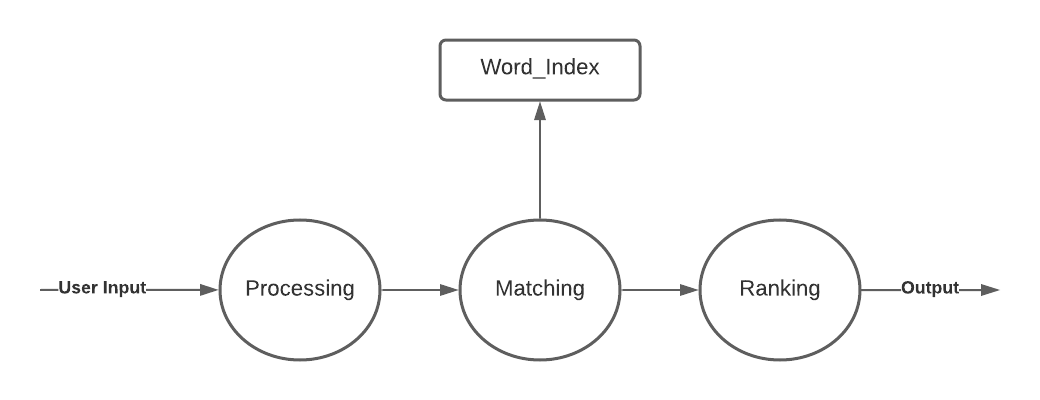
\includegraphics[width=15cm, height=8cm]{System_DFD}
		\caption{DFD of the User Interaction System}
	\end{figure}
	\subsection{Indexing}
	For fast and accurate retrieval of data, a search engine makes use of indexing. It may include components of linguistics, mathematics and other domains. These days, NLP performs a crucial role in searching for a text query.\\
	\begin{figure}[H]
		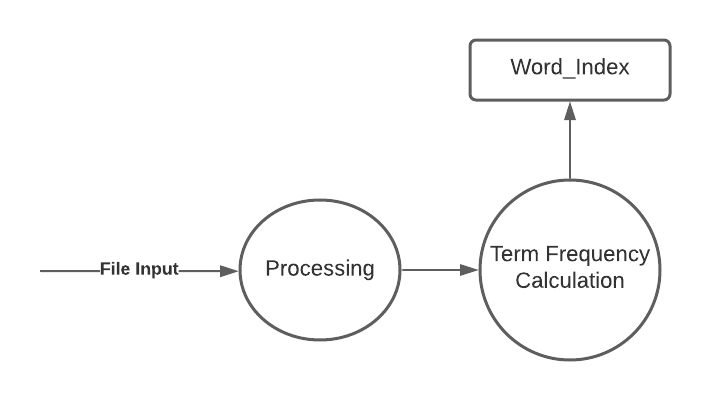
\includegraphics[width=12cm, height=8cm]{Index_DFD}
		\caption{DFD of the Indexing System}
	\end{figure}
	In this work, the index stores word level information of the texts. It maintains an index for a word and another for its stem. This is done as exact matching of a word gives a high possibility of a document being relevant to the search while matching with stems ensures that the semantic sense of the search-query is taken into account, giving lesser value to grammatical correctness.\\
	The term frequency(TF) of a word in a document is calculated during indexing as a pre-processing step. It's formula is given as : \\
	\[TF = \frac{w}{n}\]\\ 
	where,\\
	w : no. of times a word occurs in a document,\\
	n : no. of words in the document\\
	A No-SQL databsae, MongoDB, has been used for storing the index of the data. stemming is performed using a rule-based stemmer written in Python according to "A Lightweight Stemmer for Hindi" by Ramanathan and Rao \cite{hstemmer} and NLTK's implementation of the Porter Stemmer.\\
	Here is the code for indexing :
	\begin{lstlisting}
		#import relevant libraries
		from pymongo import MongoClient
		import os
		from datetime import datetime
		import pandas as pd
		
		#remove stopwords from text
		def remove_stopwords(text) :
			stopwords_set = ["|", "/", "\\", "." ,",", ")", "(", "-", "!", "~", "@"]
			for stopword in stopwords_set :
				text = text.replace(stopword, " ")
			return text
		
		#returns the stemmed version of file texts along with stem and word frequencies
		def stem_file(text) :
			text = sent_tokenize(text)
			tokens = set()
			ps = PorterStemmer()
		
			word_frequency = {}
			stem_frequency = {}
			num_words = 0
		
			for line in text :
				words = word_tokenize(line)
				num_words += len(words)
				stemmed_words = [hi_stem(word) for word in words]
				stemmed_words = [ps.stem(word) for word in stemmed_words]
				for i in range(len(words)) :
					tokens.add((words[i], stemmed_words[i], i))
		
					if words[i] not in word_frequency :
						word_frequency[words[i]] = 1
					else :
						word_frequency[words[i]] += 1
					if stemmed_words[i] not in stem_frequency :
						stem_frequency[stemmed_words[i]] = 1
					else :
						stem_frequency[stemmed_words[i]] += 1
		
		
			for word in word_frequency :
			word_frequency[word] /= num_words
			for stem in stem_frequency :
			stem_frequency[stem] /= num_words
		
			'''
				tokens -> (original_word, stemmed_word, line_number)
			'''
			return tokens, word_frequency, stem_frequency
		
		#get tokens by passing filename
		def get_stemmed_tokens(filename) :
			text = get_text(filename)
			text = remove_stopwords(text)
			tokens = stem_file(text)
			return tokens
			
		#mongodb client
		client = MongoClient()
		db = client["search_engine"]
		
		#index all files in given path
		def update_index(path) :
			for file in os.listdir(path) :
				#check if not updated
				find_file = pd.DataFrame(db.updated_logs.find({"filename" : file}))
		
				if  find_file.empty : #or timestamp greater than threshold
					tokens, word_frequency, stem_frequency = get_stemmed_tokens(path + file)
					for token in tokens :
						word = token[0]
						stemmed_word = token[1]
						line_number = token[2]
						db.word_index.insert_one({"word" : word, "stem" : stemmed_word, "filename" : file, "line_number" : line_number})
		
					for word in word_frequency :
						db.word_frequency_logs.insert_one({"word" : word, "term_frequency" : word_frequency[word], "filename" : file})
					for stem in stem_frequency :
						db.stem_frequency_logs.insert_one({"stem" : stem, "term_frequency" : stem_frequency[stem], "filename" : file})
					#mark as updated with last modified timestamp
					db.updated_logs.insert_one({"filename" : file, "time" : datetime.now()})
	\end{lstlisting}
	
	Note that all the files are indexed only once and this process does not need to be repeated for the same file. Our aim is to perform as much pre-processing at this stage as is required for fast performance during searching.
	
	\subsection{Searching}
	During this step, the search-query passes through a series of preprocessing steps. The input is broken up into tokens. These tokens are then stemmed. The stemmed tokens match the documents containing the stems from the stem\_frequency\_logs database while the unprocessed words are matched with the documents from the word\_frequency\_logs database.\\
	
	The word\_frequency\_logs matching step signifies that in relevant documents, query words match exactly with the words in those documents. Eg. Consider documents \textit{D1} and \textit{D2} and search query \textit{q}.\\
	
	\begin{flushleft}
		\textit{D1} : Ram is going to school\\
		\textit{D2} : The train goes to Washington.\\
		\textit{q} : going\\
	\end{flushleft}
	
	Since \textit{q} matches exactly with going in \textit{D1}, \textit{D1} must be more relevant to the search query.\\
	
	The stem\_frequency\_log matching step signifies that the semantic sense of the search query is preserved. Consider 2 documents \textit{D1} and \textit{D2} and search query \textit{q} :
	\begin{flushleft}
		\textit{D1} : Ram goes to school.\\
		\textit{D2} : There is a cat in the box.\\
		\textit{q} : going  \\
	\end{flushleft}
	Since the stem of 'going' and 'goes' is 'go', they will be matched together. So, \textit{q} will be matched to \textit{D1}. Hence, the semantic value of the search query is preserved by considering the stem of the search query tokens.\\
	
	It must be noted that although the examples have been given in English, a similar argument can be extended to other languages as well. \\
	
	\subsection{Ranking}
	
	The TF-IDF score has been used for ranking the matched documents. TF-IDF stands for Term Frequency Inverse Document Frequency. It is calculated for a specific term (t) in a document (d). It is calculated using the formula :\\
	\[TFIDF(t, d) = TF(t, d) * IDF(t)\]\\
	where, \\
	TF(t, d) : Term frequency of term (t) in document (d) \\
	IDF(t) : Inverse Document Frequency of term (t) considering all documents
	
	IDF can be calculated using the formula :
	\[IDF(t) = \log\frac{n}{a}\]\\
	where,\\
	n : total number of documents\\
	a : total number of documents containing term (t)\\
	
	Two separate TF-IDF scores for stem and word matchings are achieved (as explained in the previous section) and these rankings are then added for every document to get a score for each document. The documents are then sorted to get the search results.\\
	
	The code for this is as follows:\\
	
	\begin{lstlisting}
		#import required libraries
		import pandas as pd
		from pymongo import MongoClient
		import math
		import numpy as np
		
		#pymongo client
		client = MongoClient()
		db = client["search_engine"]
		
		def get_matching_docs(words, stems) :
			#get stem_freuency scores
			stem_df = pd.DataFrame(db.stem_frequency_logs.find({"stem" : {"$in" : stems}}, {"_id" : 0}))
			
			#count of documents for IDF calculation
			df_counts = pd.DataFrame(stem_df.value_counts("stem"))
			df_counts["stem"] = df_counts.index
			df_counts.reset_index(drop = True, inplace = True)
			no_docs = pd.DataFrame(db.updated_logs.find({},{"filename" : 1})).count()[0]
			df_counts.columns = ["no_data","stem"]
			df_counts["idf"] = df_counts["no_data"].apply(lambda x : math.log(no_docs / x))
			
			#merged TF-IDF scores
			merged_df = df_counts.merge(stem_df, left_on = "stem", right_on = "stem")
			merged_df["tf_idf"] = merged_df["term_frequency"] * merged_df["idf"]
			merged_df.drop(["idf", "term_frequency", "no_data"], axis = 1, inplace = True)
			
			#get word_frequency scores
			word_df = pd.DataFrame(db.word_frequency_logs.find({"word" : {"$in" : words}}, {"_id" : 0}))
			
			#counting documents for IDF calculation
			df_counts = pd.DataFrame(word_df.value_counts("word"))
			df_counts["word"] = df_counts.index
			df_counts.reset_index(drop = True, inplace = True)
			df_counts.columns = ["no_data", "word"]
			df_counts["idf"] = df_counts["no_data"].apply(lambda x : math.log(no_docs / x))
			
			#merged TFIDF scores
			merged_df_2 = df_counts.merge(word_df, left_on = "word", right_on = "word")
			merged_df_2["tf_idf"] = merged_df_2["term_frequency"] * merged_df_2["idf"]
			merged_df_2.drop(["idf", "term_frequency", "no_data"], axis = 1, inplace = True)
			return merged_df, merged_df_2
			
			#summing scores from stem and word logs
			def get_scores(words, stems) :
				df, df2 = get_matching_docs(words, stems)
				df = pd.DataFrame(df.groupby("filename").tf_idf.agg(sum))
				df.reset_index(inplace = True)
				df2 = pd.DataFrame(df2.groupby("filename").tf_idf.agg(sum))
				df2.reset_index(inplace = True)
				merged_df = df.merge(df2, how = "outer", on = "filename")
				merged_df.replace(np.nan, 0, inplace = True)
				merged_df["tf_idf"] = merged_df["tf_idf_x"] + merged_df["tf_idf_y"]
				merged_df.drop(["tf_idf_x", "tf_idf_y"], axis = 1, inplace = True)
				return merged_df
				
			#function called by flask
			def run(text) :
				tokens, a, b = stem_file(text)
				words = [token[0] for token in tokens]
				stems = [token[1] for token in tokens]
				scores = get_scores(words, stems)
				scores.sort_values("tf_idf", ascending = False, inplace = True)
				return list(scores["filename"])
	\end{lstlisting}
	
	\subsection{User Interface}
	The user interacts with the search engine using the User Interface. The API acts as a bridge between the search engine logic and the user-interface. It takes the query from the user and passes it on to the search engine logic. It also passes the results returned by the search engine back to the front-end to the user.\\
	
	The API for this project is written using Flask (Python). It runs on the local development machine and passes messages to the sear\\ch engine. The code written for the API is as follows :
	\begin{lstlisting}
		import flask
		from flask import request
		import utilities
		import Processing
		
		app = flask.Flask(__name__)
		app.config["DEBUG"] = True
		
		@app.route('/search/', methods = ["GET"])
		def search() :
			res = Processing.run(request.args.get("query"))
			return {"results" : res}
		
		if __name__ == '__main__' :
			app.run(debug = True)	
	\end{lstlisting}
	
	The API runs on a particular port on a particular IP address on the development machine network. It has a function named search which takes the "query" as an argument. It calls the \textit{run} function from the code of the previous section. It then returns as a \textit{dict} type (or a JSON Object).\\
	
	The API is called by the front-end which is an Android app (Cercher) in our case. Android is the perfect platform as it uses the GBoard virtual keyboard which enables automatic transliteration of text from Roman to Devanagri script which proves to be very use for development and testing.\\
	
	The app takes input from the user and passes it to the API. It makes network calls using the Volley library using the JsonObjectRequest class. The returned response is then populated in a RecyclerView. \\
	
	\begin{figure}[H]
		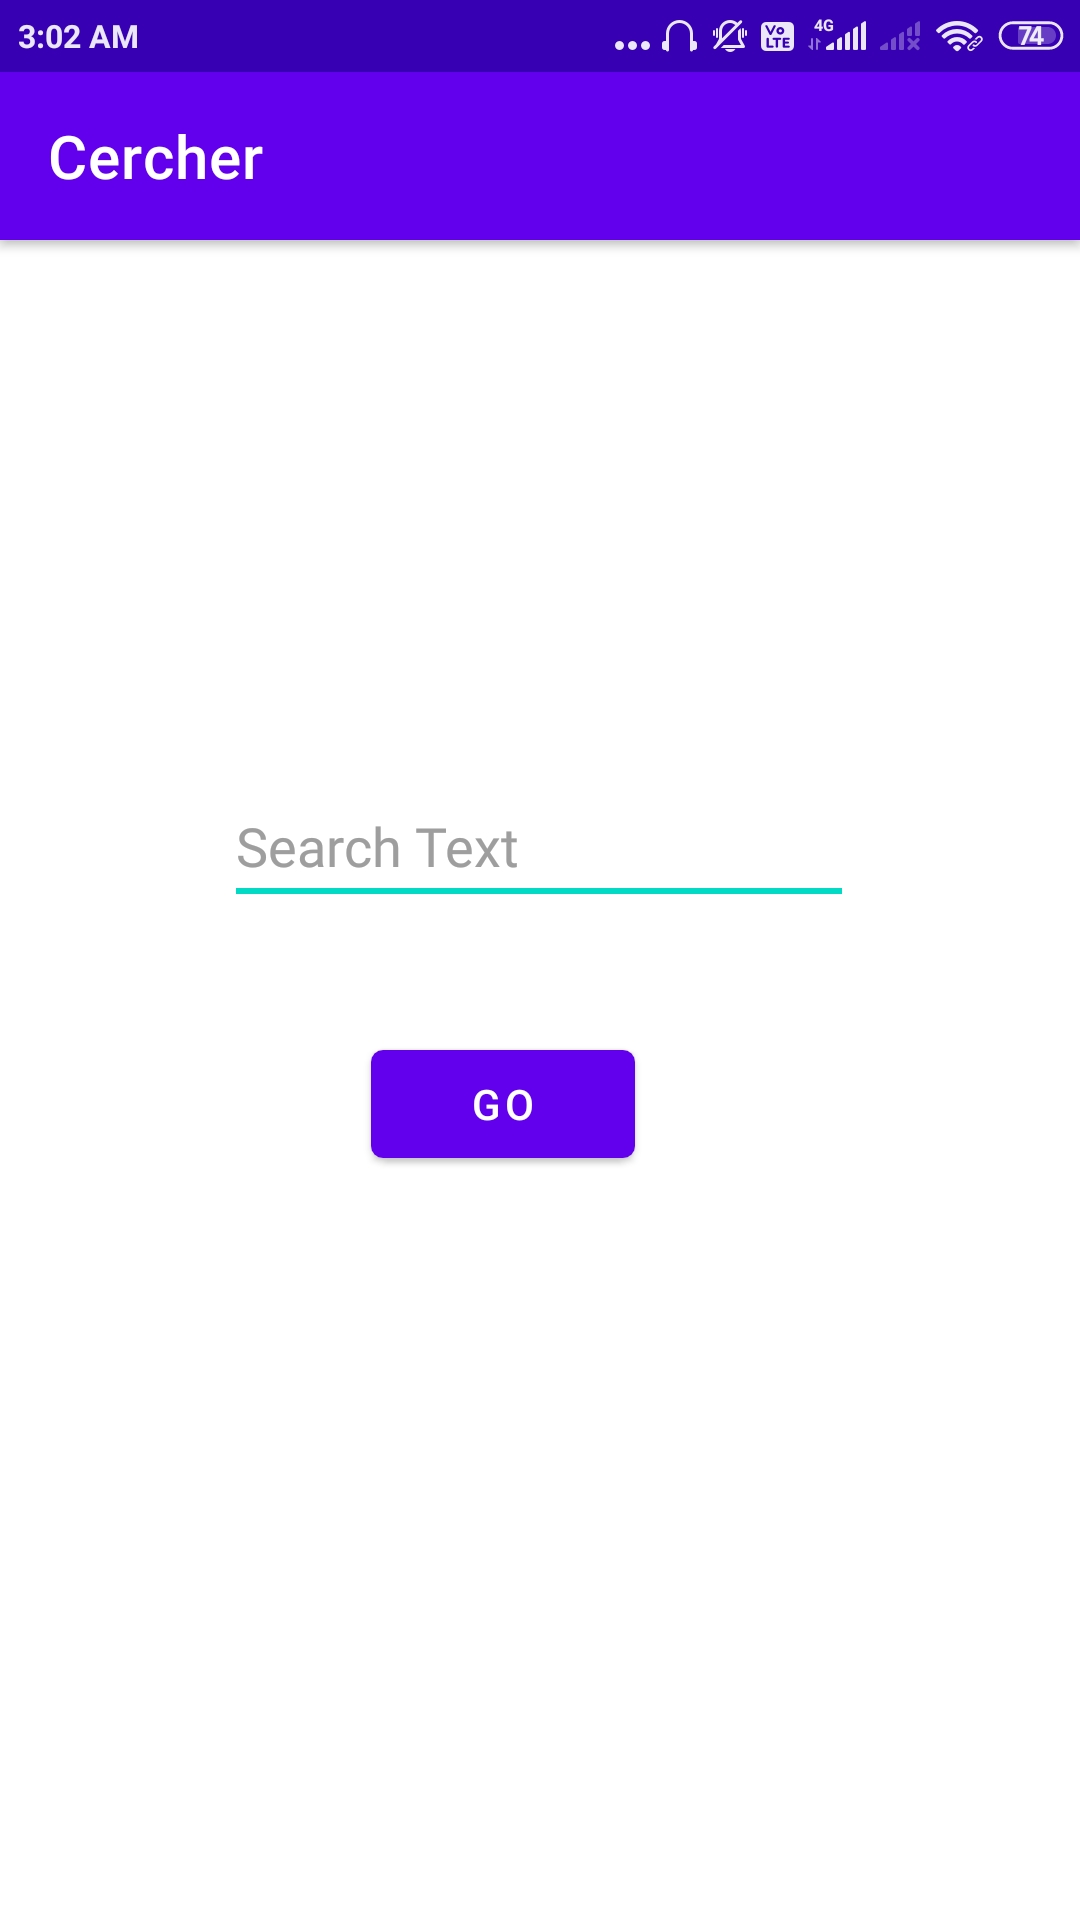
\includegraphics[width=6cm, height=12cm]{app_screen.jpeg}
		\caption{User Interface of the Android App}
	\end{figure}
	
	\pagebreak
	
	\section{Results}
	The app was tested on 2 different queries. There were 2 points to be scored. The queries were taken from different files. The size of the query was n words. For our experiment, n had the values 2, 3 and 4.\\
	
	In the experiment, the query word-count, n, was kept on increasing to understand the importance of the amount of information conveyed by each word to the search engine. When n is high, it becomes easier to find the relevant document with the excess of information. On the other hand, if the word count is too less, the search query may fail to fetch relevant results due to too little information. 
	
	If the result displayed the exact file from which the words were entered, a score of 1 is scored. If the matching file is in the top 3 relevant results, a score of 0.5 is received, else a score of 0 is given. \\
	
	For n = 2, the accuracy score was 0.8, for n = 3, the search engine had an accuracy score of 0.9. For n = 4, the score rose to 1.0. However, it must be noted that even though the search results might not have been 100\% accurate for some cases, the results that were dispayed by the algorithm were still relevant to the search query.\\
	\smallskip
	\smallskip
	\smallskip
	\smallskip
	\smallskip
	\begin{table}[H]
		\centering	
		\begin{tabular}{|c|c|c|}
			\hline
			Words & Original File & Score\\
			\begin{sanskrit}
				मुर्गा, चित्र
			\end{sanskrit} & 94.txt & 0.5\\
			\begin{sanskrit}
				सब्जी, लड़का
			\end{sanskrit} & 116.txt & 1\\
			\begin{sanskrit}
				सम्राट, नौकर
			\end{sanskrit} & 153.txt & 1\\
			\begin{sanskrit}
				कर्म, लक्ष्य
			\end{sanskrit} & 103.txt & 1\\
			\begin{sanskrit}
				अंधकार, प्रकाश
			\end{sanskrit} & 160.txt & 0.5\\
			\hline
		\end{tabular}
		\caption{Scores for n = 2}
	\end{table}
	\begin{table}
		\centering
		\begin{tabular}{|c|c|c|}
			\hline
			Words & Original File & Score\\
			\begin{sanskrit}
				महाभारत, युधिष्ठिर, भीम
			\end{sanskrit} & 2.txt & 1\\
			\begin{sanskrit}
				बीरबल, तीन, प्रश्न 
			\end{sanskrit}& 7.txt & 1\\
			\begin{sanskrit}
				बुद्ध, शिष्य, शिक्षा 
			\end{sanskrit}& 9.txt & 0.5 \\
			\begin{sanskrit}
				लड़की, श्मशान, क्रिया 
			\end{sanskrit}& 95.txt & 1\\
			\begin{sanskrit}
				सन्देश, आँख, नम 
			\end{sanskrit}& 130.txt & 1\\
			\hline
		\end{tabular}
		\caption{Scores for n = 3}
	\end{table}
	\begin{table}
		\centering
		\begin{tabular}{|c|c|c|}
			\hline	
			Words & Original File & Score\\
			\begin{sanskrit}
				महाभारत, युधिष्ठिर, ब्राह्मण, भीम
			\end{sanskrit} & 2.txt & 1\\
			\begin{sanskrit}
				बीरबल, तीन, प्रश्न, बच्चा
			\end{sanskrit} & 7.txt & 1\\
			\begin{sanskrit}
				किसान, ठोकर, पत्थर, ज़मीन 
			\end{sanskrit} & 129.txt & 1 \\
			\begin{sanskrit}
				स्वामी, विवेकानंद, माँ, महिमा
			\end{sanskrit} & 150.txt & 1\\
			\begin{sanskrit}
				देव,दानव, श्रेष्ठ, ब्रह्मा
			\end{sanskrit} & 74.txt & 1\\
			\hline
		\end{tabular}
		\caption{Scores for n = 4}
	\end{table}
	\begin{figure}
		\begin{subfigure}{0.45\textwidth}
			\centering
			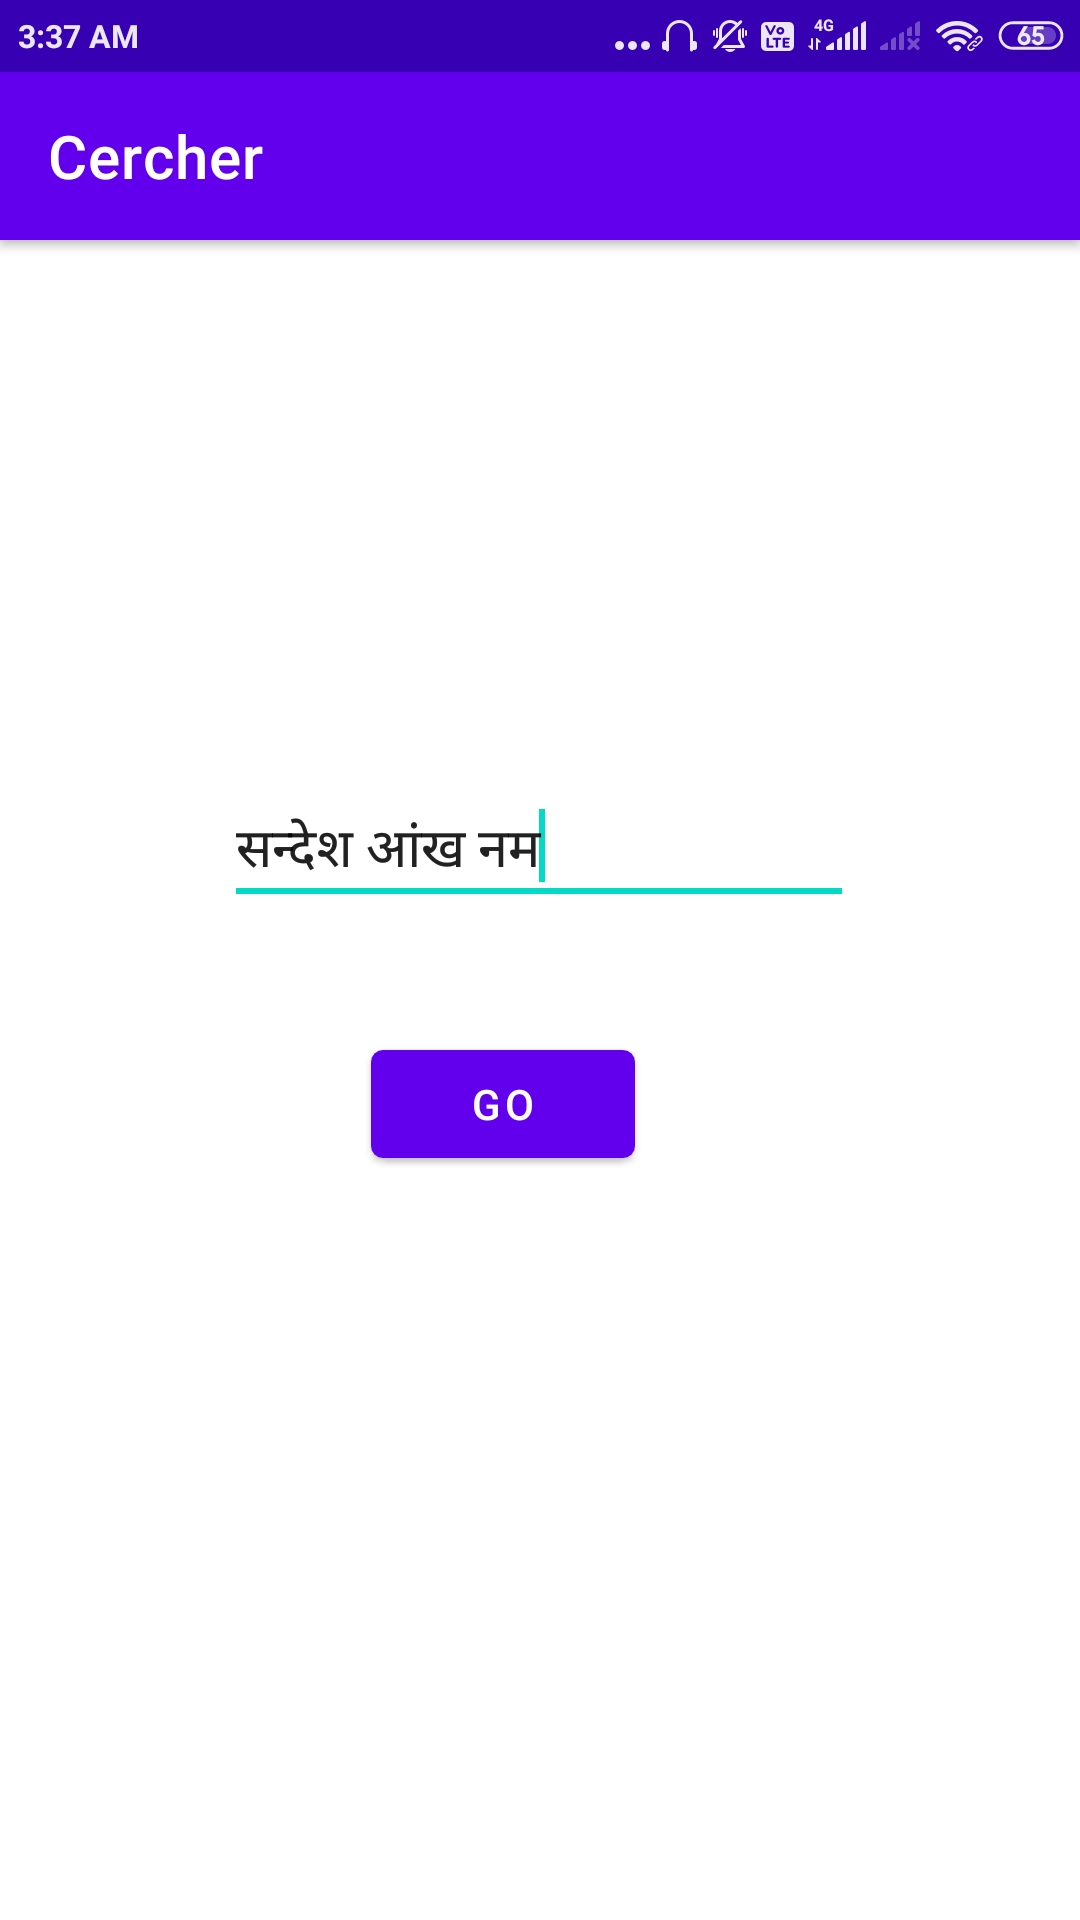
\includegraphics[width=5cm,height=8cm]{query1.jpeg}
			\subcaption{Query (from file 130.txt)}
		\end{subfigure}
		\hfill
		\begin{subfigure}{0.45\textwidth}
			\centering
			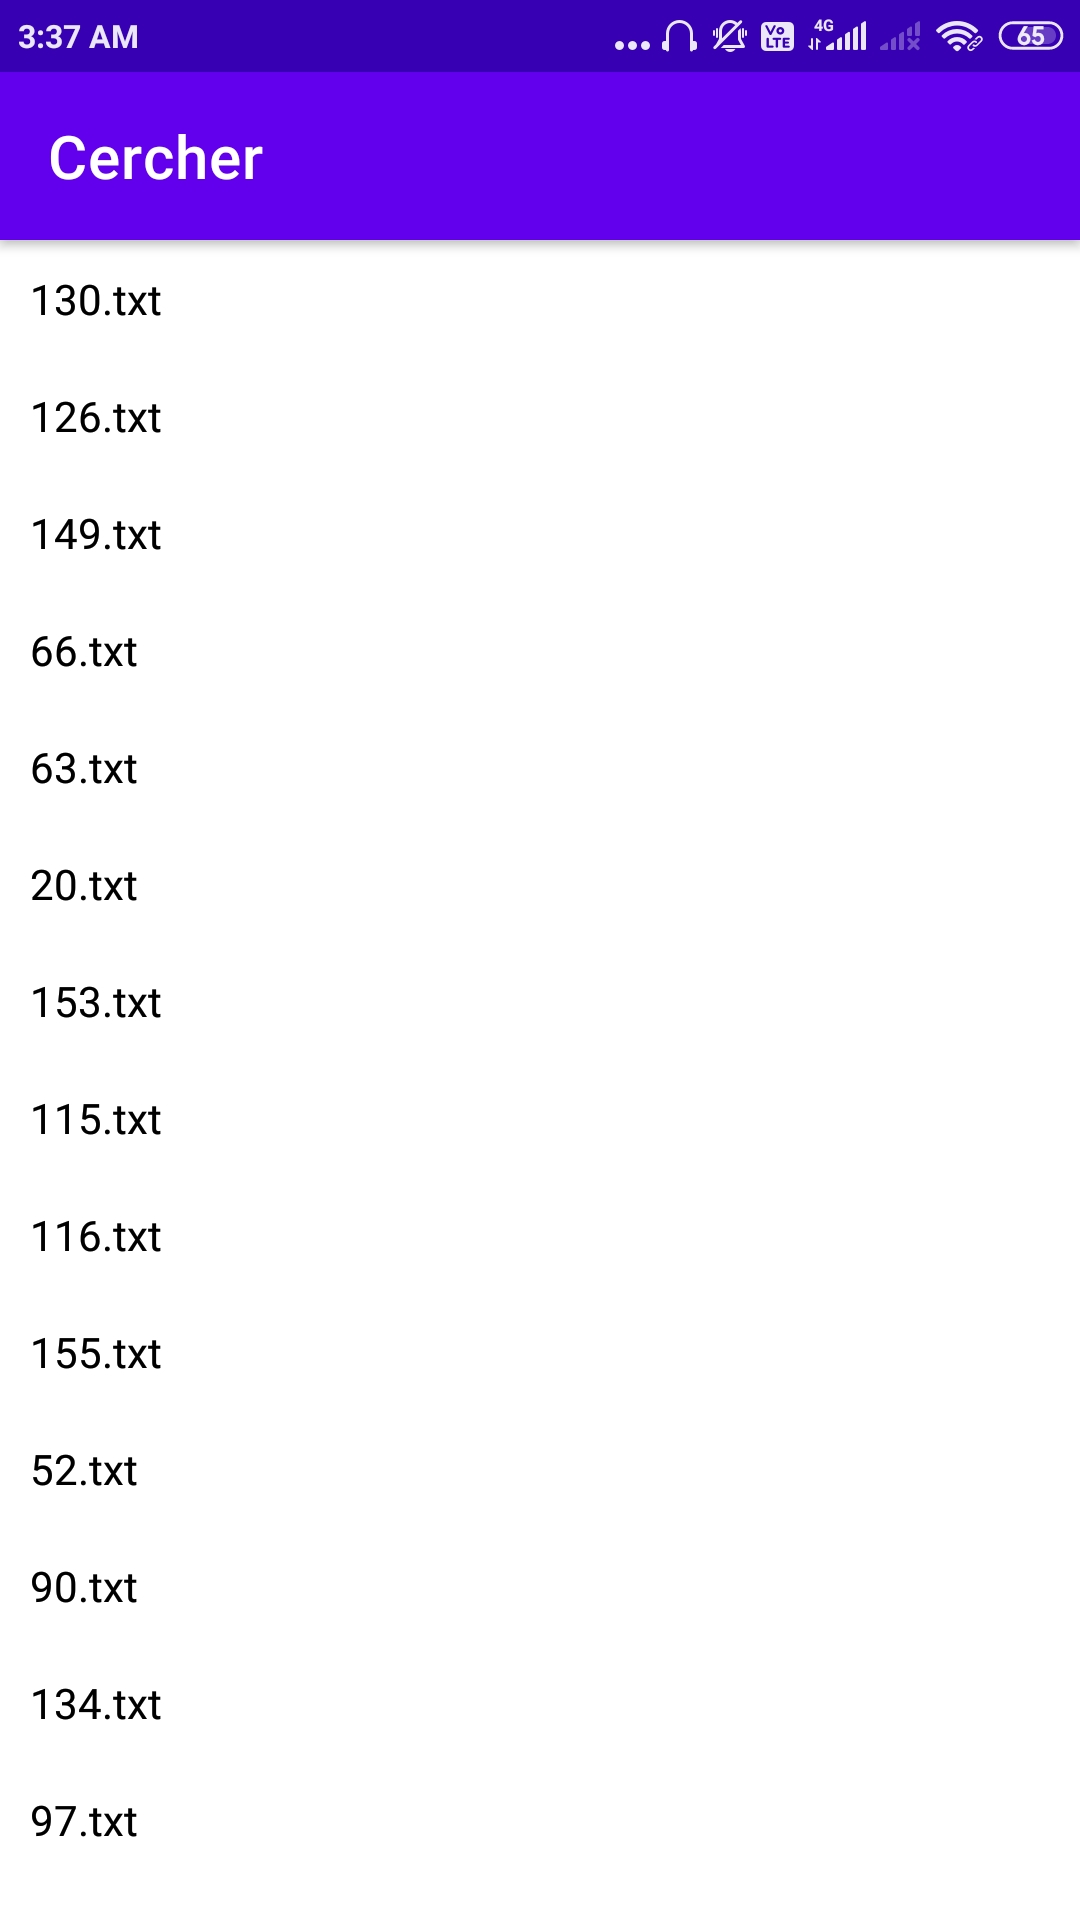
\includegraphics[width=5cm,height=8cm]{result1.jpeg}
			\subcaption{Sample Result}
		\end{subfigure}
		\caption{Sample test query using the Chercher App}
	\end{figure}
	
	\pagebreak
	\section{Conclusion}
	
	In this project we built a search engine capable of searching for documents in Hindi and English. For indexing, we performed processing and calculations in Pyhton. MongoDB was used as the database for the indexed words. The search matched relevant documents and ranked them using the TF-IDF score. \\
	
	The search query was taken as input by the Android app, Cercher, acting as the user interface. The same app displayed the search results. Volley was the network library used by the app for making network calls.\\
	
	The API, acting as the bridge between the search engine and the user interface, was written using Flask in Python.\\
	
	\newpage
	\bibliographystyle{unsrt}
	\bibliography{Refer.bib}
	
\end{document}